\todo[inline]{Update figures}
\todo[inline]{Check UC names if they are the same as in figures}
\todo[inline]{check ids of use cases}
\todo[inline]{add Save my profile UC - covers R1.4}
\todo[inline]{Add top padding for scenario tables} 
\section{Use case scenarios}
Now we are going to depict goals of users which the application will make achievable.
Figure 2.1 contains a use case diagram of the application.
A use case styled with a bold border groups together more use cases and will be further expanded.
All use cases will be structurally described by independent use case scenarios.
A scenario will contain its description only if the goal of a user is not clear from a use case's name.

\begin{figure}[h]
  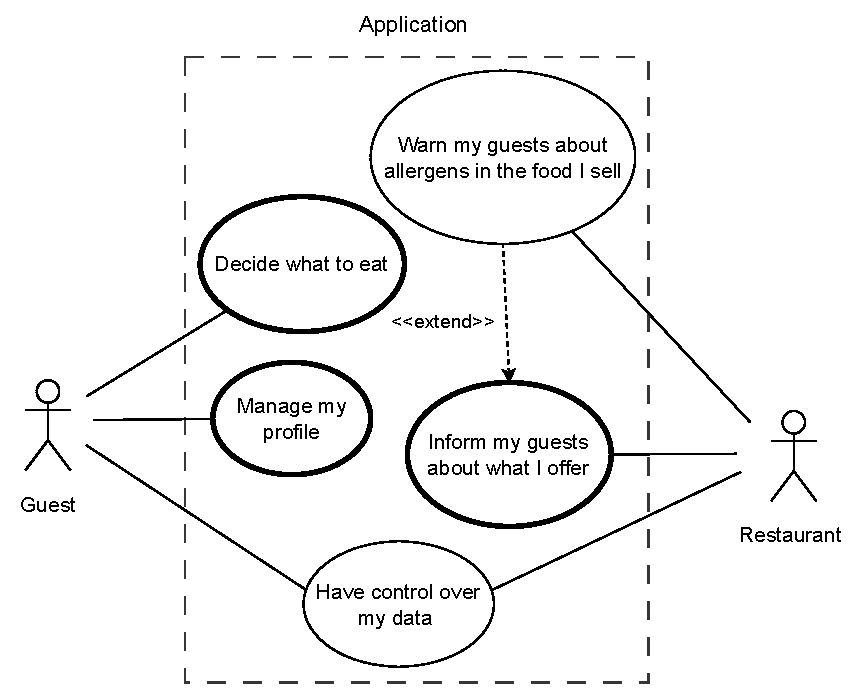
\includegraphics[width=\linewidth]{master-thesis/img/use-cases/use_cases}
  \caption{The application's use case diagram.}
\end{figure}

\newpage

\def\arraystretch{1.5}

\subsection{Guest use cases}
\todo[inline]{change name in figure}
\textbf{UC1: Decide what to order}
\begin{center}
  \begin{tabular}{| l | p{10.75cm} | }
    \hline
    Actor        & Guest \\
    \hline
    Description  & A guest comes to a restaurant and wants to choose what to order. \\
    \hline
    Covers & R1.5-R1.9, R1.16 \\
    \hline
    Precondition & The guest has opened a restaurant's menu using the application. \\
    \hline
    Postcondition & The guest is viewing a personalized menu. \\
    \hline
    Scenario     &
    \begin{minipage}[t]{\linewidth}
      \begin{enumerate}[leftmargin=*,nosep,before=\vspace{-0.575\baselineskip},after=\strut]
        \item The guest logs in to the application. \textbf{A1}
        \item The application loads the guest's profile.
        \item The application applies the guest's preferences to the menu.
        \item The application displays the menu enriched with visual clues so that the guest can see what they can and cannot eat.
        \item The guest selects to divide the menu to items they can and items they cannot eat. \textbf{A2 A3}
        \item The application restructures the menu.
      \end{enumerate}
    \end{minipage}
    \\
    \hline
    Alternatives &
    \begin{minipage}[t]{\linewidth}
      \begin{description}[nosep,after=\strut]
        \item [A1:] The guest does not log in. The guest selects what they are allergic to and what diets they follow using controls in the menu. The scenario continues with step 3.
        \item [A2:] The guest selects to sort the menu by whether they can eat an item.
        \item [A3:] The guest selects to filter out items which they cannot eat.
      \end{description}
    \end{minipage}
    \\
    \hline
  \end{tabular}
  \newline
\end{center}

\begin{figure}[h]
  \centering
  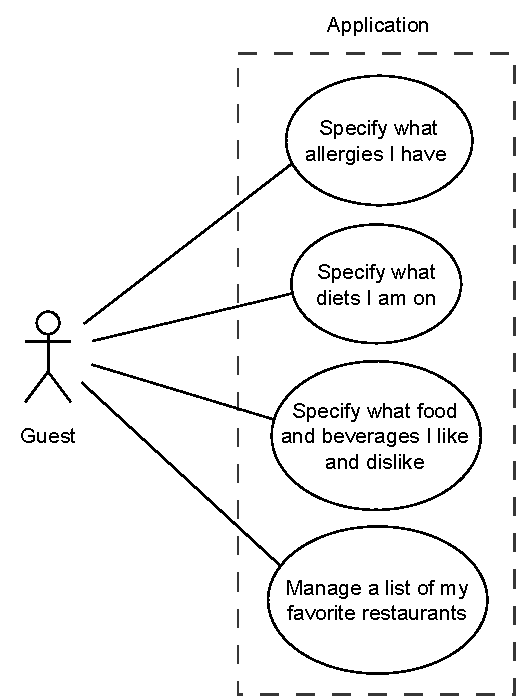
\includegraphics[width=0.62\linewidth]{master-thesis/img/use-cases/use_cases_guest_profile_management}
  \caption{Guest profile management use cases}
\end{figure}

\newpage

\todo[inline]{change name in figure}
\noindent \textbf{UC2: Specify what I am allergic to}
\begin{center}
  \begin{tabular}{| l | p{10.75cm} | }
    \hline
    Actor         & Guest \\
    \hline
    Covers        & R1.1 \\
    \hline
    Precondition  & The guest is logged in to the application. \\
    \hline
    Postcondition & The guest's profile contains data about what the guest is allergic to. \\
    \hline
    Scenario      &
    \begin{minipage}[t]{\linewidth}
      \begin{enumerate}[leftmargin=*,nosep,before=\vspace{-0.575\baselineskip},after=\strut]
        \item The guest opens their profile.
        \item The application displays options for what a person can be allergic to.
        \item The guest selects options based on what they are allergic to. \textbf{A1}
        \item The guest presses a button for saving their profile.
        \item The application updates the guest's profile.
      \end{enumerate}
    \end{minipage}
    \\
    \hline
    Alternatives &
    \begin{minipage}[t]{\linewidth}
      \begin{description}[nosep,after=\strut]
        \item [A1:] Some of the options are selected because the guest has already specified them in the past.
      \end{description}
    \end{minipage}
    \\
    \hline
  \end{tabular}
  \newline
\end{center}

\noindent \textbf{UC3: Look up online what a restaurant offers today}
\todo[inline]{add a path where the guest is not authenticated}
\todo[inline]{add a branch where the menu gets translated}
Covers R1.10-R1.12, R1.15, R1.16
\todo[inline]{change main path to find a restaurant by its name - clicking a link on a webpage as alternative}
\begin{center}
  \begin{tabular}{| l | p{10.75cm} | }
    \hline
    Actor        & Guest \\
    \hline
    Description  & A guest is at home or on their way to a restaurant and wants to know what the restaurant serves at the moment. \\
    \hline
    Covers & Rx.x \\
    \hline
    Scenario     &
    \begin{minipage}[t]{\linewidth}
      \begin{enumerate}[leftmargin=*,nosep,before=\vspace{-0.575\baselineskip},after=\strut]
        \item The guest visits the restaurant's webpage and clicks on a link which takes them to the application. \textbf{A1 A2 A3}
        \item The application displays the restaurant's detail which contains a list of its menus.
        \item The guest selects a menu.
        \item The application displays the menu.           
      \end{enumerate}
    \end{minipage}
    \\
    \hline
    Alternatives &
    \begin{minipage}[t]{\linewidth}
      \begin{description}[nosep,after=\strut] 
        \item [A1:] The guest selects a restaurant in the overview screen from UC4.
        \item [A2:] The guest specifies the IRI of the restaurant. 
        \item [A3:] The guest scans a QR code on a printed menu which takes them to the application.
      \end{description}
    \end{minipage}
    \\
    \hline
  \end{tabular}
  \newline
\end{center}

\newpage

\todo[inline]{Make the figure bigger - increase height, make bubbles bigger}

\begin{figure}[h]
  \centering
  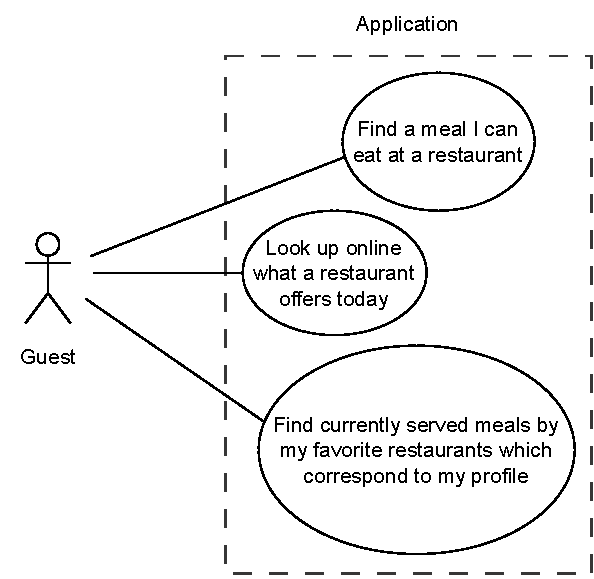
\includegraphics[width=0.62\linewidth]{master-thesis/img/use-cases/use_cases_guest_menu_viewer}
  \caption{Guest menu viewing use cases}
\end{figure}

\todo[inline]{change name (also in figure) to "Find currently served meals by my favorite restaurants which I can eat"}
\noindent \textbf{UC4: Find currently served meals by my favorite restaurants which correspond to my profile}
Covers R1.14
\begin{center}
  \begin{tabular}{| l | p{10.75cm} | }
    \hline
    Actor        & Guest \\
    \hline
    Description  & A guest wants to know what do their favorite restaurants currently have to offer. \\
    \hline
    Covers & Rx.x \\
    \hline
    Precondition & The guest is logged in to the application. \\
    \hline
    Postcondition & The guest sees a list of their favorite restaurants with selected items from their menus. \\
    \hline
    Scenario     &
    \begin{minipage}[t]{\linewidth}
      \begin{enumerate}[leftmargin=*,nosep,before=\vspace{-0.575\baselineskip},after=\strut]
        \item The application displays an overview of what the guest's favorite restaurants currently serve. \textbf{A1}\textbf{A2} \textbf{A3}
      \end{enumerate}
    \end{minipage}
    \\
    \hline
    Alternatives &
    \begin{minipage}[t]{\linewidth}
      \begin{description}[nosep,after=\strut]
        \item [A1:] The restaurants do not currently serve anything. The application displays a text with this information.
        \item [A2:] The overview is empty because the guest has not added any of their favorite restaurants yet. The application displays instructions on how to add a restaurant to the list.
        \item [A2:] A restaurant has no valid menu published at the moment. The application displays a text with this information close to the restaurant's name.
      \end{description}
    \end{minipage}
    \\
    \hline
  \end{tabular}
  \newline
\end{center}

\newpage

\noindent \textbf{UC5: Specify what diets I am on}

Covers R1.2
\begin{center}
  \begin{tabular}{| l | p{10.75cm} | }
    \hline
    Actor       & Guest \\
    \hline
    Covers & Rx.x \\
    \hline
    Scenario    &
    \begin{minipage}[t]{\linewidth}
      \begin{enumerate}[leftmargin=*,nosep,before=\vspace{-0.575\baselineskip},after=\strut]
        \item The guest opens their profile and navigates to a section for managing diets.
        \item The application displays a screen with a list of previously specified diets by the guest. \textbf{A1}
        \item The guest presses a button labeled as "Add diet".
        \item The application displays a search bar.
        \item The guest starts typing the name of a diet into the search bar.
        \item The application suggests diets which contain the given input in their name.
        \item The guest selects the desired diet and presses an "Add" button. \textbf{A2}
        \item The application adds the specified diet to the guest's profile. \textbf{A3}
        \item The guest repeats steps 3 to 8 until they have specified all of the diets they are on.
      \end{enumerate}
    \end{minipage}
    \\
    \hline
    Alternatives &
    \begin{minipage}[t]{\linewidth}
      \begin{description}[nosep,after=\strut]
        \item [A1:] The list is empty because the guest has not specified any diets yet. The application displays a text containing this information.
        \item [A2:] The application does not recognize the diet which the guest is trying to specify. The guest creates a public issue in the application's repository with a request to add the desired diet to the application.
        \item [A3:] The diet the guest has specified is already contained in the guest's profile. The application informs the guest about this fact and their profile is not altered.
      \end{description}
    \end{minipage}
    \\
    \hline
  \end{tabular}
  \newline
\end{center}

\noindent \textbf{UC6: Have control over my data}
\begin{center}
  \begin{tabular}{| l | p{10.75cm} | }
    \hline
    Actor        & Guest \\
    \hline
    Description  & A guest wants to specify where should the application store and read their data. \\
    \hline
    Covers & Rx.x \\
    \hline
    Scenario     &
    \begin{minipage}[t]{\linewidth}
      \begin{enumerate}[leftmargin=*,nosep,before=\vspace{-0.575\baselineskip},after=\strut]
        \item The guest navigates to a page for managing data storage options.
        \item The application provides a list of places where it can store data.
        \item The guest selects one of the options.
        \item The application starts using the selected place for storing and reading the guest's data.
      \end{enumerate}
    \end{minipage}
    \\
    \hline
  \end{tabular}
  \newline
\end{center}

\newpage

\noindent \textbf{UC7: Specify what food and beverages I like and dislike}
Covers R1.3
\begin{center}
  \begin{tabular}{| l | p{10.75cm} | }
    \hline
    Actor    & Guest \\
    \hline
    Covers & Rx.x \\
    \hline
    Scenario &
    \begin{minipage}[t]{\linewidth}
      \begin{enumerate}[leftmargin=*,nosep,before=\vspace{-0.575\baselineskip},after=\strut]
        \item The guest opens their profile and navigates to a section for managing food preferences.
        \item The application displays a screen with two lists, one containing the foods which the guest likes and the other containing the foods which the guest dislikes. \textbf{A1}
        \item The guest presses a button labeled as "Add food" at the end of the list of foods which they like. \textbf{A2}
        \item The application displays a search bar.
        \item The guest starts typing the name of a food into the search bar.
        \item The application suggests foods which contain the given input text in their name.
        \item The guest selects the desired food and presses an "Add" button. \textbf{A3}
        \item The application adds the specified food to the guest's profile. \textbf{A4}
        \item The guest repeats steps 3 to 8 until they have specified all of their food preferences.
      \end{enumerate}
    \end{minipage}
    \\
    \hline
    Alternatives &
    \begin{minipage}[t]{\linewidth}
      \begin{description}[nosep,after=\strut]
        \item [A1:] Either one or both of the lists are empty because the guest has not specified any of their preferences yet. The application displays a text which informs the guest about this fact.
        \item [A2:] The guest presses a button labeled as "Add food" at the end of the list of foods which they dislike.
        \item [A3:] The application does not recognize the food which the guest is trying to specify. The guest creates a public issue in the application's repository with a request to add the desired food to the application.
        \item [A4:] The guest's profile already contains the specified food. The guest is informed about this fact and their profile is not altered.
      \end{description}
    \end{minipage}
    \\
    \hline
  \end{tabular}
  \newline
\end{center}

\newpage

\todo[inline]{check in other use cases whether I used ',' between A1 and A2}
\noindent \textbf{UC8: Manage a list of my favorite restaurants}
Covers R1.13
\begin{center}
  \begin{tabular}{| l | p{10.75cm} | }
    \hline
    Actor    & Guest \\
    \hline
    Covers & Rx.x \\
    \hline
    Precondition & The guest is logged in to the application. \\
    \hline
    Postcondition & A restaurant is added to the list of the guest's favorite restaurants. \\
    \hline
    Scenario &
    \begin{minipage}[t]{\linewidth}
      \begin{enumerate}[leftmargin=*,nosep,before=\vspace{-0.575\baselineskip},after=\strut]
        
        \item The application displays a list of the guest's favorite restaurants. \textbf{A1 A2}  
        \item The guest presses the button for adding a new restaurant to the list.
        \item The application displays a text input field.
        \item The guest starts typing the name of the restaurant. \textbf{A3}  
        \item The application suggests restaurants which contain the specified text in their name to the user. 
        \item The guest clicks on a restaurant's name. \textbf{A4}
        \item The application adds the selected restaurant to the list. \textbf{A5}
      \end{enumerate}
    \end{minipage}
    \\
    \hline
    Alternatives &
    \begin{minipage}[t]{\linewidth}
      \begin{description}[nosep,after=\strut]
        \item [A1:] The guest is viewing a restaurant's detail. The guest presses the button for marking the restaurant as their favorite. The application adds the restaurant to the guest's profile. \textbf{A1.b}
        \item [A1.b:] The restaurant is already contained in the guest's profile and pressing the button removes the restaurant from it.
        \item [A2:] The list is empty because the guest has not added any restaurants yet. The application displays a text with this information.
        \item [A3:] The guest specifies the restaurant's IRI. \textbf{A3.b}   
        \item [A3.b:] The IRI which the guest specified is not valid. The application informs the guest about this fact and the scenario continues with step 4.
        \item [A4:] The application did not find the desired restaurant because it does not use our application. The application displays a text saying that it was not able to find any restaurants by the specified name. The scenario ends.
        \item [A5:] The guest's profile already contains the restaurant by the specified name. The guest is informed about this fact and their profile is not altered.
      \end{description}
    \end{minipage}
    \\
    \hline
  \end{tabular}
  \newline
\end{center}

\newpage